
%What can we do?
\section{The impact of the difference}\label{eva}
In the previous sections we 
specified how existing interpretations of formulas in \nthreelogic differ in their handling of implicit quantification. Here, 
we take a closer look at these differences. 
% and address research questions (iii) and (iv) from the introduction:\todo{incorporate more or remove}
% \begin{itemize}
%   \item[(iii)] How often does the conceptual difference between the handling of implicit quantification of \nthreelogic lead to conflicting interpretations 
%   of formulas used in practical applications?
%  \item[(iv)] Which kinds of constructs cause these conflicting interpretations in practice and how likely is it that a file containing these constructs is actually 
%  subject to the problem?
% \end{itemize}
% %
How do they impact 
practical cases? In which kinds of applications are they relevant?
In order to answer these questions, we implemented the attribute grammar introduced above and tested for several formulas
whether the two interpretations we formalised 
differ on these examples. %We have applied this program to different datasets.
An explanation of the implementation, the datasets used and the results of our tests -- quantitative and qualitative -- is given below. 

\subsection{Implementation}\label{imp}
For our evaluation we have implemented the attribute grammar as specified above. 
In order to stay close to our format, we used the Utrecht University Attribute Grammar (UUAG) and its compiler 
the Utrecht University Attribute Grammar Compiler (UUAGC)~\cite{uuag}. This framework enables the user to specify attribute grammars which 
then get translated to Haskell code and can be used in all kinds of applications. All additional applications and functions were written in Haskell.
%
% 
% As programming language we have chosen Haskell and the grammar itself is written
% using the Utrecht University Attribute Grammar Compiler (UUAGC)~\cite{uuag}. This framework enables the user to specify attribute grammars in a similar format as above, 
% the so-called  Utrecht University Grammar (UUAG), which then gets translated to Haskell code and can be used in all kinds of applications. 


For every \nthree formula, our program produces the syntax tree of the translated core logic formula as well as its string representation in our two 
interpretations.
% , ie  
% according to Cwm, and according to EYE. 
We furthermore implemented a function which compares these translations. Note that in \nthree, 
especially in Cwm's interpretation, every file needs to be treated as one formula. This is because the conjunction is done by
putting triples after each other. It makes a difference whether 
\[
 \texttt{\{:a :b \{:c :d ?x\}\} => \{:e :f :g\}. }
\]
is followed by
\[
  \texttt{:s :p \{\textbf{?x} :p :o\}.} \text{\quad or \quad}  \texttt{:s :p \{\textbf{?y} :p :o\}.}
\]
In the first case Cwm's interpretation puts the quantifier for the variable \texttt{?x} on the top formula; in the second case it is inside the premise of the rule.
We therefore cannot give the meaning of the first implication without taking its context into account. Our function thus always 
compares the meaning of an entire file and then displays the concrete differences between interpretations. All code can be accessed at \url{https://github.com/IDLabResearch/N3CoreLogic}.
% We therefore always compare 
%the interpretation of an entire file.

%In the previous section we defined an attribute grammar in order to obtain the different interpretations of \notationthree formulas. 
% To use the grammar presented in the last section in practical applications it has to be transferred into programme code.
% With the goal of providing a tool to compare the differences between the interpretations, we implemented this grammar
% using the Utrecht University Attribute Grammar Compiler (UUAGC)~\cite{uuag}. 
% This compiler takes an attribute grammar written in a special format, the Utrecht University Grammar (UUAG) as input and translates it 
% to Haskell code which then can be used for
% further programming. 
%In this chapter we give a brief introduction into the formalism in general, our use of it and our implementation of a comparison tool for different interpretations
%of \nthree
%in Haskell. 


%Question: which impact does the different scoping have for real use cases? 

\subsection{Datasets used}\label{data}
To test whether the differences described above can be observed in practical applications,
we used two kinds of datasets: a test dataset of the reasoner 
EYE and several datasets used in previous research projects.

The \emph{EYE dataset}\footnote{Accessible at \url{https://github.com/josd/eye/tree/master/reasoning/}. Our tests are based on the version of October 15, 2017.} 
%
%To get an idea of the impact of the difference in interpretations
%To test the impact of the different interpretations cwm and EYE support for N3 formulas, we chose different datasets:
%\begin{description}
is a collection of test cases for the EYE reasoner.
Some of the tests were created to challenge the reasoner (e.g. parsing of nested expressions, scoping of blank nodes and universals)
and are therefore rather artificial, 
 but the majority of test files was either sent by users of the reasoner to explain problems they had or are minimal examples of practical use cases from different parties.
 In that sense 
 the content of the dataset 
 reflects a big variety of applications created by different users.
 At the moment we tested, the dataset contained 359 \nthree files in 50 folders of which 303 contained implicitly 
quantified universal variables. 
As the latest version of EYE does not support that feature, the tests cases do not include explicit quantification. 

\hyphenation{ORCA DiSSeCt}
The \emph{Project datasets} contain rules we specified in previous projects, in particular: 
%We chose this dataset because of the big number of contributors. 
 %semonstrate there test cases, in that sense the tests are representatibe.
 %\item[cwm dataset]
the projects \emph{ORCA (Ontology based Reasoning for nurse Call)} \cite{ORCA,ORCA2}, \emph{Facts4Workers (Factories for Workers)} \cite{arndt_ruleml_industry_2016} 
and \emph{DiSSeCt (Distributed Semantic software solutions for complex Service Composition)}
\cite{ruleml2017}. 
%
The rules of the 
\emph{ORCA dataset}\footnote{This 
project was in cooporation with an industry partner and the results might be used in a product. The rules are therefore not public.}
 are written to perform an optimized version of OWL-RL reasoning and to follow a complex decision tree which, depending on the set-up and the 
current situation of a hospital, assign the best staff member to answer a patient call. We further explain that in Section~\ref{orca}.
%\end{description}
%
The aim of the rules from the \emph{Facts4Workers} use-case\footnote{Available at \url{https://github.com/IDLabResearch/Facts4Workers/tree/master/n3}.}
is to deal with the diverse infrastructure of modern factories in which different machines are able to perform a huge variety of tasks.
These tasks are described via rules which can be combined to fulfil a desired goal. The idea behind that is further explained in Section~\ref{restdesc}.
%
The last set of rules\footnote{Available at \url{https://github.com/IDLabResearch/data-validation}. },
used in the project \emph{DiSSeCt}, is designed to check \rdf datasets for user-specified constraints. These are the topic of Section~\ref{validation}.
%
We chose these datasets because they were produced to be used in practical rather complex applications and not to merely test the reasoner. 
To ensure compatibility with EYE
the datasets do not make use of explicit quantification.

For our tests, we selected only the files which contain universal variables. For the ORCA dataset this selection contained 130 files, for Facts4Workers 25 files,
and for DiSSeCt 84 files.


\subsection{Results}\label{results}
\begin{table}
\begin{center}
\begin{tabular}{rrrr}
\hline
\bf dataset& \bf \#files & \bf \#differences & \bf percentage\\
\hline
 \bf EYE &303 & 81 &  27\%\\
 \bf F4W &25 & 12 &  48\% \\
 \bf ORCA & 130& 27 & 21\%\\
 \bf DiSSeCt & 84&50&  60\%\\
 \hline
 \bf Total & 542 & 179& 31\%\\
 \hline
\end{tabular}
\end{center}
\caption{Results of tests for differences in the interpretations of \nthree files. By \#differences we mean the number of files which are interpreted differently 
by the two reasoners.\label{result}}
\end{table}
For the datasets introduced above, we  tested whether the reasoners interpret every file in the exact same way, ie whether the two 
core logic translations produced by our 
software were the same (accepting differences in the naming of variables and in the order of universal and of existential quantifiers on the same 
level of a formula), 
or whether we can identify differences. The results 
are displayed 
in Table~\ref{result}. We see that every dataset contains files for which the interpretation differs between Cwm and EYE. Nevertheless, 
the portion of affected files varies per dataset and depends on the nature of the data. We have identified three kinds of constructs which can be related with disagreements 
in the interpretation:
\begin{description}
  \item[Proofs] formulas which represent a formal \emph{proof}, ie an explanation of the derivation steps leading to a conclusion; % using the \nthree proof vocabulary~\cite{Proof};  %as introduced in Section~\ref{proofintro};
  \item[Built-ins] formulas which contain built-in functions which have a special meaning for one or both reasoners;
  \item[Nesting] formulas which, without using built-in functions, cite graph patters, act on them or perform
reasoning about rules.
\end{description}
Before taking a closer look at the distribution of these three cases in the different datasets, 
we explain what we mean by \emph{proofs}, \emph{built-ins} and \emph{nesting} in more detail.

%The DiSSeCt dataset contains a very high number of proofs.





%It is too late to change the meaning of blanks, it is not too late for universals.

%\subsection{Qualitative Results}
%Where did we find the differences?
%Mostly in proofs. But also rule producing rules in ORCA. Give examples.
\subsubsection{Proofs}\label{pro}
In Section~\ref{proofintro} we already explained that there is a proof vocabulary defined for \nthree. The reasoners Cwm and EYE 
make practical use of this vocabulary: From both reasoners the user can request a formal proof as an explanation of the derivations made. Such a proof contains 
all proof steps applied on the data provided to the reasoner leading to the output of the reasoner. We will further explain these steps and the underlying calculs in Chapter~\ref{proof}.
For our tests in the current section, it is more important, how exactly these steps are represented:
%
% When drawing conclusions from data, both reasoners are able to provide an explanation for their derivations. For that they both use the \nthree proof 
% vocabulary\footnote{\url{https://www.w3.org/2000/10/swap/reason\#}}  
% created in the context of the Semantic Web Application
% Platform (SWAP)~\cite{SWAP}. 
%The vocabulary makes it possible to express proof steps performed by the reasoners. 
%
While Cwm proofs only contain explicit universal 
quantification and are therefore out of scope for our current evaluation, EYE proofs employ implicit universal quantification in nested constructs. 

We already saw an example
of an inference proof
step in Listing~\ref{example2}, in 
% another 
% An example proof step is given in
Listing~\ref{proof22} we display another kind a proof step,
\begin{lstlisting}[
  float=t,
  caption={Representation of a proof step. },
  label=proof22]
§\scriptsize\textcolor{gray}{
@prefix\quad  : <http://example.org/ex\#>.}§
§\scriptsize\textcolor{gray}{@prefix r: <http://www.w3.org/2000/10/swap/reason\#>.}§

 <#lemma1> a r:Extraction;
  r:gives { {:s :p ?x1} => {:s :pp ?x1}. };
  r:because [ a r:Parsing; r:source <rules.n3> ].
\end{lstlisting}
% 
% We see the proof step of 
an \texttt{r:Extraction}. This corresponds to conjunction elimination from common first-order calculi: 
if a bigger conjunction is known 
to be correct, so are its conjuncts. %These can be used in further derivations.
Here, this example step 
is based on another step, a \texttt{r:Parsing}, ie reading information from a file which in the example has the symbolic name \texttt{rules.n3}.
The proof steps yield the formula \begin{equation}\texttt{\{:s :p ?x1\} => \{:s :pp ?x1\}.}\label{fo}\end{equation} indicated by the predicate \texttt{r:gives}. 
Interesting from a structural point of view is  
that the formula appears in a formula expression.  For Cwm the variable \texttt{?x1} is therefore universally quantified in this expression. We get the interpretation:
\[
 \texttt{<L1> gives <}\forall \texttt{x. <s p x>}\rightarrow\texttt{<s pp x> >.}
\]
Since the file from which the formula stems contains Formula~\ref{fo} this interpretation is correct in this context. For 
EYE all variables are quantified on top level,  we get: % the interpretation:
\[
\forall \texttt{x. <L1> gives < <s p x>}\rightarrow\texttt{<s pp x> >.}
\]
Yet, if we consider the meaning of the predicate \texttt{r:gives} which indicates the consequences we can draw from the reasoning steps, then this interpretation is also right:
from the fact that Formula~\ref{fo} appears in our data we can for every \texttt{x} conclude that $\texttt{ < <s p x>}\rightarrow\texttt{<s pp x> >.}$ 
Hence in this case the differences 
in the interpretations do not have practical consequences even if the proofs are used for further reasoning.

\nthree reasoning mostly depends on rules containing universal variables. Like in the example, most proofs list the parsing and selection of such rules and 
are therefore often
subject to the problem described. In our datasets, this is the case for all proofs. 

% When a formula is cited
% 
% \texttt{ <\#Lemma1> r:gives \{\{:s :p ?o\}=>\{:s :pp ?o\}\}.}
% 
% Is that ever right? Here I should come to a conclusion.
%\subsection{Findings}
\subsubsection{Built-ins}
% \begin{lstlisting}[
%   float=t,
%   caption={Rule including the predicate \texttt{log:includes}. },
%   label=includes]
% §\scriptsize\textcolor{gray}{PREFIX log: <http://www.w3.org/2000/10/swap/log\#>}§
% §\scriptsize\textcolor{gray}{PREFIX\qquad :\quad<http://example.org/ex\#>}§
%  
% {{:a :b :c} log:includes {:a :b ?x}}
%     => {:d :e :f}. 
% \end{lstlisting}
Another big group of differences in the interpretations of a formula can be observed in connection with built-in functions.
%\rv{I disagree with this phrasing. The problem does not seem to be the built-in functions, but rather the interpretation of formula expressions (which happen to occur more frequently with certain built-ins).}
Both reasoners, Cwm and EYE, provide 
a set of predicates with predefined meanings\footnote{Available at  \url{https://www.w3.org/2000/10/swap/doc/CwmBuiltins} for Cwm, and 
\url{http://eulersharp.sourceforge.net/2003/03swap/eye-builtins.html} for EYE.}
which can be used to, for example, deal with lists (\texttt{rdf:first}), to compare terms (\texttt{log:equalTo}) or to do calculations (\texttt{math:product}). 
Some built-in predicates are reasoner-specific. Using these leads to different reasoning results. % for 
%formulas containing built-ins. %the use of such a predicate can cause differences in the reasoning results,
But even if a
predicate is supported by different reasoners, we often get differences in connection with their usage.
This is because many built-ins deal with graphs or graph patterns. % and do therefore, if used in implications, cause differences in the interpretation. 
% When looking at those differences, we have to keep in mind that some built-in functions are only supported by one of the two reasoners.
% %Files containing these predicates can---regardless of the interpretation of implicit universals---not be exchanged by the two reasoners.
% Since this already causes a compatibility problem on its own---a reasoner cannot produce the same result as another if it is not aware of the special meaning of a predicate---it does not make sense to look deeper into 
% these kinds of examples.
% \todo{less strong}


%Not all of the built-in functions are supported by both reasoners and their use can on its own already lead to differences in the reasoning result. 
%But there are also built-in functions defined for both reasoners which, used in the premise of a rule, can cause disagreements between reasoners. 
As an example consider the built-in predicate \texttt{log:includes}\footnote{Prefix \texttt{log:<http://www.w3.org/2000/10/swap/log\#>.}} % which is defined for both reasoners. In Listing~\ref{includes} we see an example rule 
%applying that built-in function. % \texttt{log:includes}. 
which is supported by both reasoners and compares formula expressions. A triple \texttt{ A log:includes B.} is correct
iff the terms \texttt{A} and \texttt{B} are formula expressions and the triples occuring in \texttt{B} also occur in \texttt{A}. \texttt{ \{:a :b :c\} log:includes \{:a :b :c\}.} 
is correct 
while \texttt{ \{:a :b :c\} log:includes \{:a :b :o\}.}
is not.  %In Listing~\ref{includes} we see an
The following rule contains a triple using \texttt{log:includes} in its antecedent: 
\begin{multline}\notag
 \texttt{\{\{:a :b :c\} log:includes \{:a :b ?x\}\}}
   \texttt{ => \{:d :e :f\}.} 
\end{multline}
The shape of this triple is similar to the examples 
given before with the difference that instead of \texttt{:o} or \texttt{:a}, the object of the triple in the right-hand side formula expression is the universal \texttt{?x}. 
Cwm interprets this formula as
\begin{multline}\notag
 \texttt{<}\forall \texttt{x. <a b c> includes <a b x>{}>} \rightarrow\texttt{<d e f>.}
\end{multline}
%And 
Since it is not true that for every \texttt{x} the expression \texttt{<a~b~x>} is included in \texttt{<a b c>} -- think 
for example in the case above, $\texttt{x}=\texttt{o}$ -- %
the consequent of the formula is not derived in Cwm. Opposed to that, EYE understands
\begin{multline}\notag
 \forall \texttt{x.}\texttt{ <{} <a b c> includes <a b x> {}>} \rightarrow \texttt{<d e f>.}
\end{multline}
Here, the antecedent of the implication is fulfilled for $\texttt{x}=\texttt{c}$. EYE derives the new triple \texttt{d~e~f.} 
%Since built-in functions which are
%only supported by one of the reasoners cause a compatibility problem anyway, we discuss here an example of a built-in which is implemented in both reasoners.
The different interpretation of universals changes the reasoning result.


% \begin{verbatim}
%  {{:b :a :c. :e :d :f. :h :g :i. :k :j :l} 
%  log:includes {:k :j :l. ?X :d ?Z}} 
%    => {:logi1 :result true}.
% \end{verbatim}
\begin{lstlisting}[
  float=t,
  caption={Example rule using a nested graph (taken from the project Facts4Workers). },
  label=F4W]
§\scriptsize\textcolor{gray}{@prefix http: <http://www.w3.org/2011/http\#>.}§
§\scriptsize\textcolor{gray}{@prefix math: <http://www.w3.org/2000/10/swap/math\#>.}§
§\scriptsize\textcolor{gray}{@prefix\hspace{0,65cm}:\quad<http://example.org/ex\#>.}§
 
{  
 {?machine :hasProblem ?problem.} :eventId ?eid.
 (?eid 1) math:sum ?nid
}
=>
{
 _:request http:methodName "POST";
           http:requestURI "https://f4w/actions";
           http:body       ("stop" ?machine).
      
 {?machine :stoppedBecause ?problem.} :eventId ?nid.
}. 
\end{lstlisting}
\begin{lstlisting}[
  float=t,
  caption={Interpretation of Listing~\ref{F4W} according to Cwm. The occurrences of variable \texttt{?problem} are understood as two different variables. },
  label=F4Wcwm]
§$\forall$§ m. §$\forall$§ i. §$\forall$§ i2.
<
 §$\forall$§ p.
 <m hasProblem p> hasId i.
 (i 1) sum i2 
> 
§$\rightarrow$§
<
 §$\forall$§ p1. §$\exists$§ r. 
 r methodBame 'POST'. 
 r requestURI 'https://f4w/actions'.
 r body ('stop' m).
 <m stoppedBecause p1> eventid i2. 
>
\end{lstlisting}
\subsubsection{Nesting}\label{nest}

Our examples contain a third kind of difference:
rules which either operate on other rules or on graph structures. Many examples for this can be found in the 
ORCA dataset where rule-producing rules are applied (this will be further explained in Section~\ref{orca}) but also  in the Facts4Workers dataset, where formula expressions 
refer to events.
A (shortened) example of such a reference in a rule is shown in Listing~\ref{F4W}. 

In this example we can perform actions on machines. Such actions can for example be to start or stop the machine, but also to simply do an observation of a problem. Each action performed gets an event id. 
The rule from the example expresses that, if a problem is observed, the very next action to be performed is to stop the machine (here via an http-call). Note, that the different actions or events in this example 
are expressed by formula expressions which contain universal variables. While in EYE the two occurrences of the variable \texttt{?problem} in Line 6 and Line 15  co-refer -- here, 
the universal quantification of implicit universals is always on top level -- this is not the case for Cwm whose interpretation is displayed in Listing~\ref{F4Wcwm}.
We clearly see that the two occurrences of  
\texttt{?problem} are understood as two different variables. The meaning of the rule differs between reasoners 
and the implementation of this use case  does not work with Cwm. 

% Another interesting observation we make when looking closely  to the rule is that the problem we described for \texttt{?problem} does not occur for the variable \texttt{?machine}, a variable which occurs next to 
% \texttt{?problem} in the formula expressions. The reason for that is that \texttt{?machine} also occurs in a list in the consequent of the rule which lifts the quantifier of the variable one level upwards to outside of the rule. The interpretation of this variable does not differ between the two reasoners.


% \begin{multline}\notag
% \forall \texttt{m.}\forall \texttt{i.} \forall \texttt{i2.}
% \\ \texttt{<}\forall \texttt{p.<m hasProblem p> hasId i.(i 1) sum i2>}\\
% \rightarrow\texttt{<}\forall \texttt{p1.}\exists
% \\\texttt{r. r methodBame ``POST''.}\\ \texttt{ r requestURI ``https://f4w/actions''.}\\\texttt{ r body (``stop m).
% <m stoppedBy p2> eventid i2 
% >}
%\end{multline}




\subsubsection{Distribution of Cases}\label{cases}
Having seen examples for common cases causing differences in the interpretation of \nthree formulas, we return to the numbers of Table~\ref{result}.
%: How are these
%cases distributed within the datasets? 
These numbers depend on the nature of the datasets and the constructs they contain: If a dataset does not contain proofs at all our implementation will also not find
 any problems related to proof constructs there. 
The same holds for the two other kinds of potentially problematic constructs we describe above. 
% On the other hand,
% it is not always the case 
%As these numbers depend on the nature of our datasets, 
We therefore show in Figure~\ref{datasets} how many files contain proofs, built-ins and nesting of any kind\footnote{In that context we define
nesting as containing at least one formula expression occurring in another one as in the example
$\texttt{:a :b \{:c :d \{:e :f :g.\}.\}.}$
where \texttt{\{:e :f :g.\}} is nested.} (dark blue). 
Next to that information, we also display, how many of these constructs actually lead to conflicting interpretations
%and for how many files one of these constructs causes conflicting interpretations 
(light blue). %In Appendix~\ref{}
% To understand the reasons causing the different interpretations in our tests, we analyse their nature:
% How many proofs do they contain? How often do we find nesting of any kind 
% (regardless of the universals involved), and 
% how many of them contain built-ins? The answers to these questions are displayed in Figure~\ref{datasets} (dark blue part). %The figure shows for each dataset how many of the afore mentioned cases it contains. 
%
Note that the cases we consider are overlapping: proofs can contain built-ins, 
files can have deeply nested formula expressions at one place and use built-ins at other places. Due to the nature of proofs, every proof file is also subject to nesting. 
\begin{figure}
 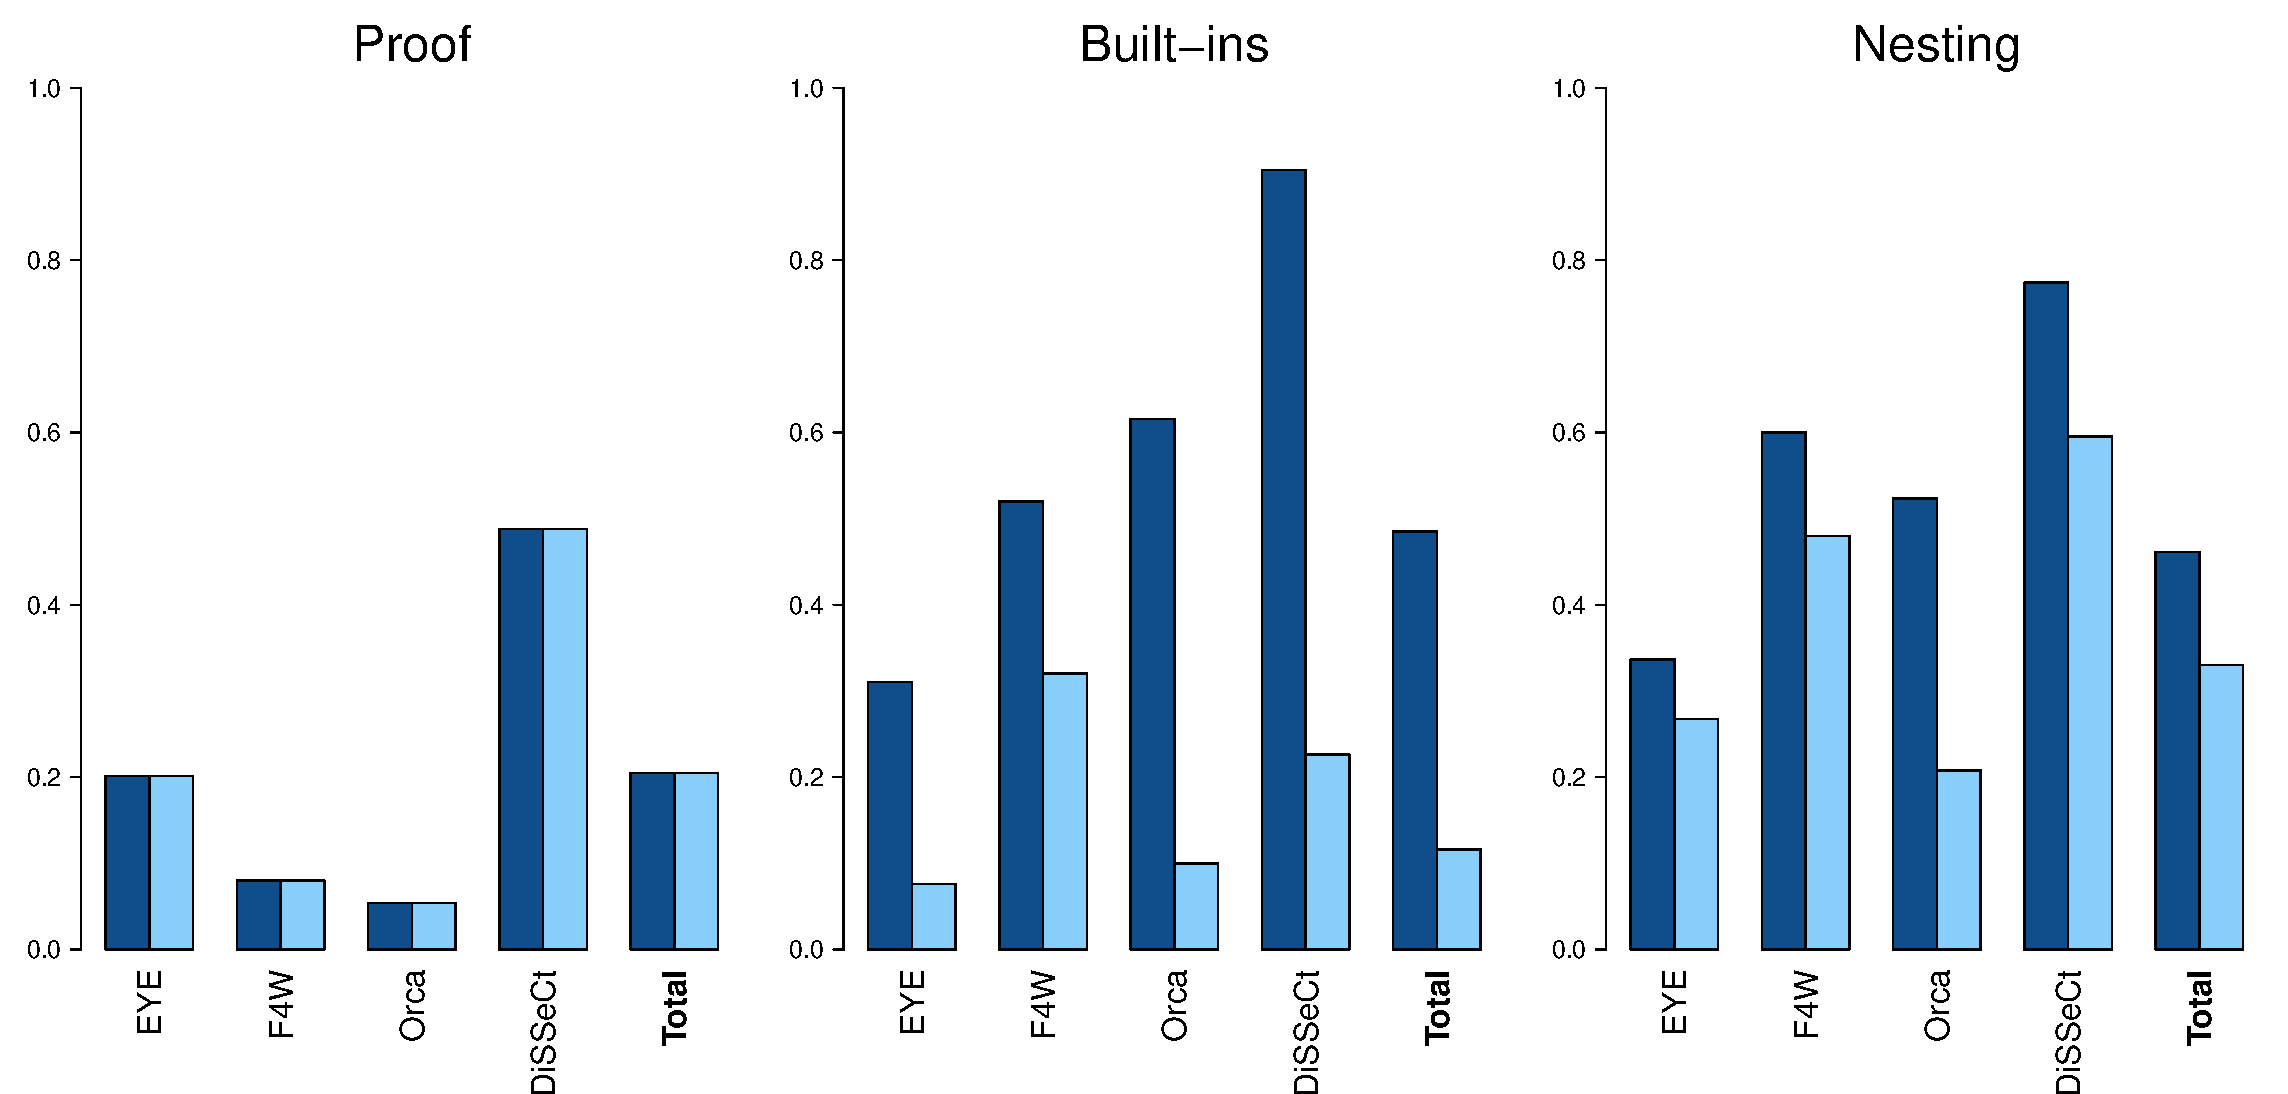
\includegraphics[width=0.95\textwidth]{Rplot06.pdf}
 \caption{Distributions of proofs, built-ins and nesting in datasets. The share in dark blue always represents the files containing the respective feature while light blue is used to represent the cases
 where the feature leads to different interpretations.\label{datasets}}
% \rv{I think this graph can still improve.
%   First, the light blue does not add any information;
%   remove it, so the focus is on the actual information
%   (which makes the figure much more intuitive,
%   as we don't need to read the caption anymore now).
%   Second, consider a different color for the total column.}
% \rv{Can we add extra information,
%   namely the number of cases where there are interpretation differences?
%   So Proofs/EYE now shows 20\%,
%   can we split this into two stacked bars
%   where one is green (no diffs) and one is red (diffs)?}
\end{figure}

We already mentioned earlier that proofs containing universal variables cause conflicting interpretations and that in our examples all proofs contain such variables.
As a consequence, the dataset containing most proofs, the DiSSeCt data set, is also the one having the highest share of diverging interpretations.
%which we also expect to be the case for most proofs in general.
%Taking a closer look
%As mentioned above all proof files containing universals and rules cause disagreements which also explains why for
% Having that in mind, it is easy to understand why the DiSSeCt data set
% which consists by 50\% of proofs is also the one having the highest share of diverging interpretations. 
For the other kinds of constructs we discussed, built-in functions and nesting, we take a closer look at the numbers appearing in 
Figure~\ref{datasets} below where we also explain how the values were calculated. %Additionally we explain, how they were calculated.
% The share of built-ins causing differences is rather small, for nesting, which includes the cases of proofs and built-ins, it is rather high. 
% Below, we discuss the last two cases in detail. 

%Since almost half of the DiSSeCt data set consists of proofs, it is not surprising that here we also found the highest number of disagreements (60\%).
% Considering Figure~\ref{datasets} it is not surprising that for the DiSSeCt dataset we found the highest share of disagreement between interpretations (60\%):  
% almost half of the dataset consists of proofs. 
% These cause different interpretations whenever rules and universals are involved. 
% The DiSSeCt dataset additionally 
% contains a very high number of built-ins which 
% are often another source of disagreement. 

%  The figure additionally contains the shares of these files where the observed feature (ie proofs, built-ins or nesting) causes problems (light blue). 



\subsubsection*{Disagreements per Formula Type}
In order to understand how many of the built-ins present in our datasets are causing problems, 
we extended the attribute grammar by additional attributes. We give the definition of these attributes in Appendix~\ref{cbi}. Here, 
we only want to briefly discuss the idea: If a triple has a built-in function in predicate position we test whether subject and object of that triple contains universal 
variables.
If this is the case, we next need to know where exactly the interpretation according to Cwm quantifies these variables. If all these universal variables are quantified
on a higher level than the $\text{parent}_c$ level of the built-in then the built-in construct itself is not 
causing conflicting interpretations. 

In Figure~\ref{datasets} where the numbers calculated by that method are displayed 
in the middle we already see that in many cases the presence of a built-in construct in a data set does not cause problems. 
To better understand how likely this presence of a built-in constructs causes contradicting interpretations we display the numbers from above in another way.
Figure~\ref{builtins} shows in how many of the files containing built-in functions at least one of the built-in functions occurs in a construct which causes 
contradictory interpretations.
%
% To better understand how likely it is that in a file containing built-in constructs, these constructs also cause contradicting interpretations, we display the numbers 
% presented in the middle of Figure~\ref{datasets} in another way: 
% This information is already captured in the 
% attribute grammar we introduced in Section~\ref{n3}: attribute $s$ collects for all nodes the universal variables which are quantified on the node itself or 
% any higher level. A universal variable occurring in subject or object position of a built-in \texttt{b} is subject to the problem described above if it is not contained 
% in the value of $\texttt{b}.s$. 
% % To know that we can use the syntax tree and the 
% % information which is already collected by attribute $s$ (discussed in Section~\ref{n3}). This attribute passes in the syntax tree which variables are 
% % already quantified on a higher level.
% 
% which test 
% for every subject or object of a built-in predicate whether it contains universal 
% variables which Cwm quantifies %does not quantify %in Cwm's interpretations is not 
% %quantified 
% %on the $\text{parent}_c$ 
% either on the level of the built-in itself or any lower level. The definition of these attributes can be found in Appendix~\ref{cbi}.
%  
%  The results of our tests are displayed in Figure~\ref{builtins}. For each dataset we show the percentage of files containing 
% at least one built-in construct 
% which the two reasoners interpret differently compared to all files containing built-ins.
We see that for the whole dataset and most subsets approximately a quarter of all 
files with built-ins contains at least one critical construct. Only in the Facts4Workers dataset this share is higher.
This has to do with the fact that in that project one specific built-in is used very often: 
% which can be explained by
% the fact that here the built-in 
 The built-in \texttt{e:whenGround}\footnote{See \url{http://eulersharp.sourceforge.net/2003/03swap/log-rules.html\#whenGround}. }
 %is used in many rules to 
 tests whether its subject contains variables or is ground and calls the object if the latter is true. This built-in is implemented in EYE for
 a few very specific use cases. We expect that users employing such special predicates are aware of the fact that their rules only work with one specific reasoner.
 The cases counted here are therefore less critical for the problem that files written for use cases of the Semantic Web which rely on interoperability are interpreted 
 contradictory by different reasoners.
 

\begin{figure}
 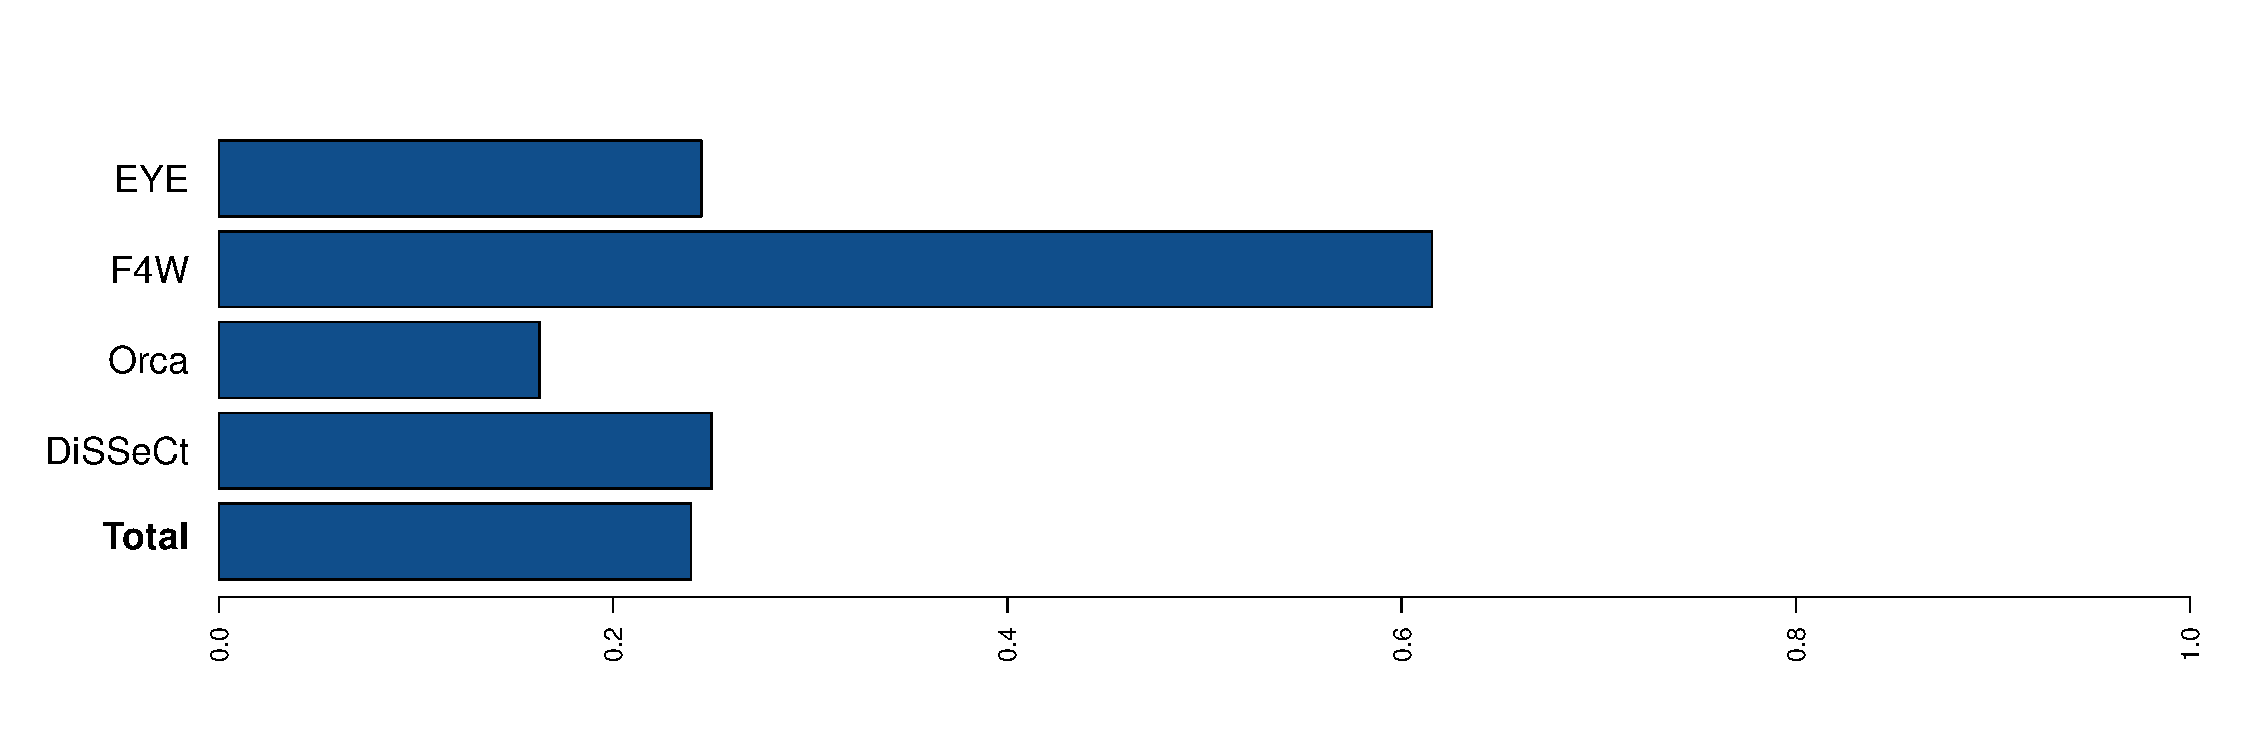
\includegraphics[width=\textwidth]{Rplot01.pdf}
 \caption{Share of files containing built-ins causing conflicting interpretations in
 files containing built-ins. Only in a quarter of all files containing built-ins 
 these occur with deeply nested universals.
\label{builtins}}
\end{figure}  
 
A similar figure as the one above can be produced for nested formulas. We display the share of formulas being subject of a nesting problem in all 
formulas containing nesting in Figure~\ref{onlynests}. In Figures~\ref{datasets} and \ref{onlynests} we understand a formula as nested if it contains 
a graph construct in a graph construct (ie a formula in nested brackets \texttt{\{}$\ldots$\texttt{\{}$\ldots$\texttt{\}}$\ldots$\texttt{\}}). 
As a nesting construction leading to the problems described in this section we understand any nested construct containing a universal variable 
for which the quantifier according to Cwm is %where Cwm quantifies this universal 
on any other level than the top level. This rather broad definition qualifies all differences listed in Table~\ref{result} as subject to a nesting problem and these 
numbers are also used for the two figures.
% Figure~\ref{datasets} 
% uses these numbers.
% 
% Similarly to the case just seen, we can ask how many files  of our set of formulas containing nesting have different interpretations caused by deeply nested variables. Since all problems we consider 
% in Table~\ref{result} are caused by different interpretations of nested variables -- as this is how we constructed our tests -- we used these numbers to generate Figure~\ref{onlynests}. 
% % Here we see how many
% of the files including nesting have conflicting interpretations. 
We observe that, when deep nesting is already present in a file, we suffer from conflicting interpretations in 72\% of the cases.
This is not very surprising since most nested graphs occur in rules which most likely also contain universals, but this figure shows once again, that when using nested graphs, users need to be careful 
with universal variables.

\subsubsection*{Categorisation of Errors}
As a last point in this subsection we display how the different problem types are distributed over the files counted in Table~\ref{result}.   
The reasons for conflicting interpretations of a formula 
can be overlapping. 
% Especially if we have a proof it can be useful to know whether conflicting interpretations are only 
% caused by the proof vocabulary which normally uses graphs -- 
% these cases are rather harmless -- or if built-ins with deeply nested universals in their
% subject or object, or another occurrence of deeper nested universals are involved. 
% a universal variable To test how deeply nested in the formula 
% the deepest nested variable occurs we defined other attributes which we discuss in~\ref{nested}. 
% We measure the depth of a universal variable as one plus the number of formula expressions its quantifier is enclosed in when translating the \nthree formula 
% to its core logic translation according
% to Cwm. If a variable does not occur in a file at all, it has depth 0. Looking back to the formulas we have already seen, we can for 
% example say that in Formula~\ref{fff} the variable \texttt{?y} has depth 2 while \texttt{?x} has depth 1. 
% To calculate the maximum depth of a quantifier in a formula 
% we used attributes. 
% The definition of these can be found in~\ref{nested}.
% 
% Because of the nature of the proof we know that if the maximum depth of the universal quantifiers is two or lower, then the only reason for conflicting interpretations 
% is the use of the 
% predicate \texttt{r:gives} which has a graph as object. If the maximum depth of universal variables is bigger than two, 
% we know that the conflict 
%  found in the proof is more serious and caused by a deeper nesting in one of the formulas occurring in the object of \texttt{r:gives}. 
%
To be able to show a distribution we separate them in disjoint groups as follows: 
\begin{description}
\item[Built-in Group] Every formula containing a built-in construct which leads to contradictory interpretations
% built-in functions used in connection with formula 
% expressions containing universals
is counted as such even if this construct occurs in a proof or additionally contains nested graph constructs without built-ins.
\item[Proof Group]
Every proof formula for which the reason of the contradictory interpretations is only the proof structure itself. 
That means that the formula does not belong to the \emph{Built-in Group} and that the results of the proof 
steps -- ie the \textit{result} part in the triples \texttt{<\#lemma> r:gives \{} \textit{result} \texttt{\}} -- do not contain any universal variables which 
Cwm quantifies on a level which is nested inside these results.
% not belonging to the \emph{Built-in Group}
% for which the results of all proof steps 
% do not contain nested graphs with universal variables which Cwm quantifies on that level are counted as a proof.
\item[Nesting Group]
Every formula not belonging to the two groups above is counted as a nested formula.
\end{description}

To test whether conflicting interpretations are caused by built-ins, we used the attributes introduced above. 
% For the \emph{Proof Class} we needed to determine whether the only reason 
% for conflicting interpretations is the nature of the  proof structure -- in which case the formula is member of the \emph{Proof Class} -- 
% or whether there are universal variables which Cwm quantifies on a deeper level
% than the level of the formula expression cited by \texttt{r:gives} -- these formulas are captured in the \emph{Nesting Class}. 
The method to determine whether a formula representing a proof belongs to the \emph{Nesting Class} or the \emph{Proof Class}  is discussed in Appendix~\ref{nested}. 


\begin{figure}
 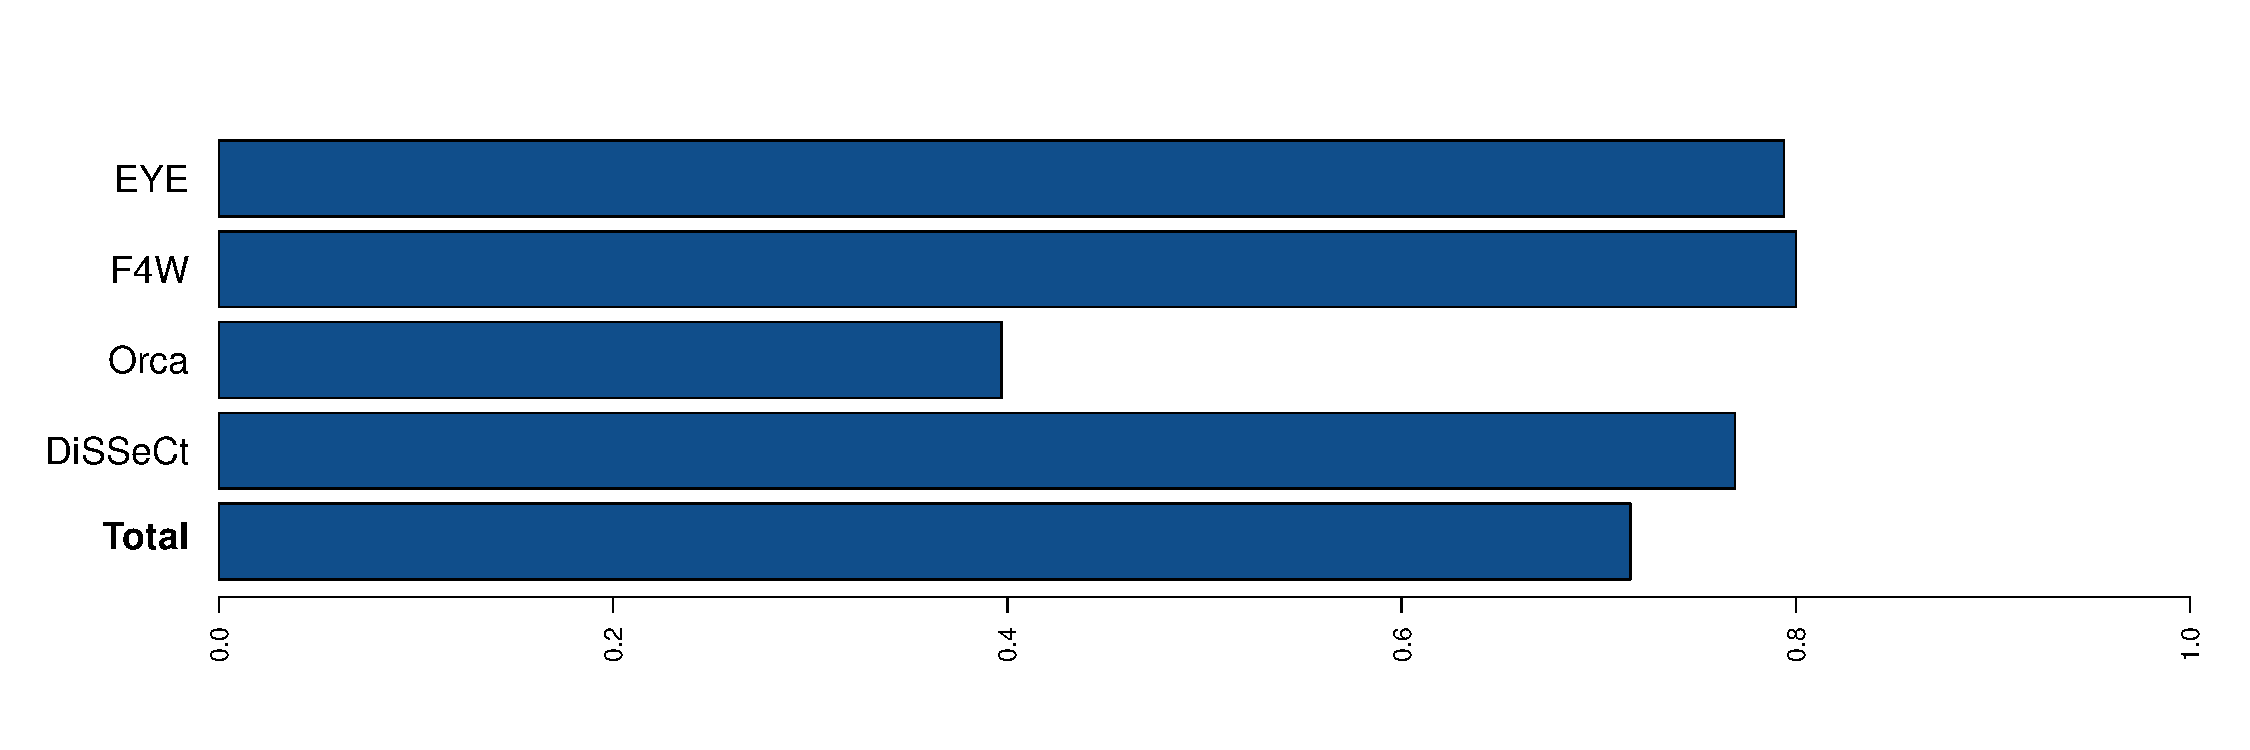
\includegraphics[width=\textwidth]{Rplot03.pdf}
 \caption{Share of files causing conflicting interpretations in
 files which have nested expressions. 72\% of the files containing nesting are interpreted differently by both reasoners.
\label{onlynests}}
\end{figure}

% \begin{figure}%[htb]
%     \centering
%     \begin{minipage}[t]{0.49\linewidth}
%         \centering
%         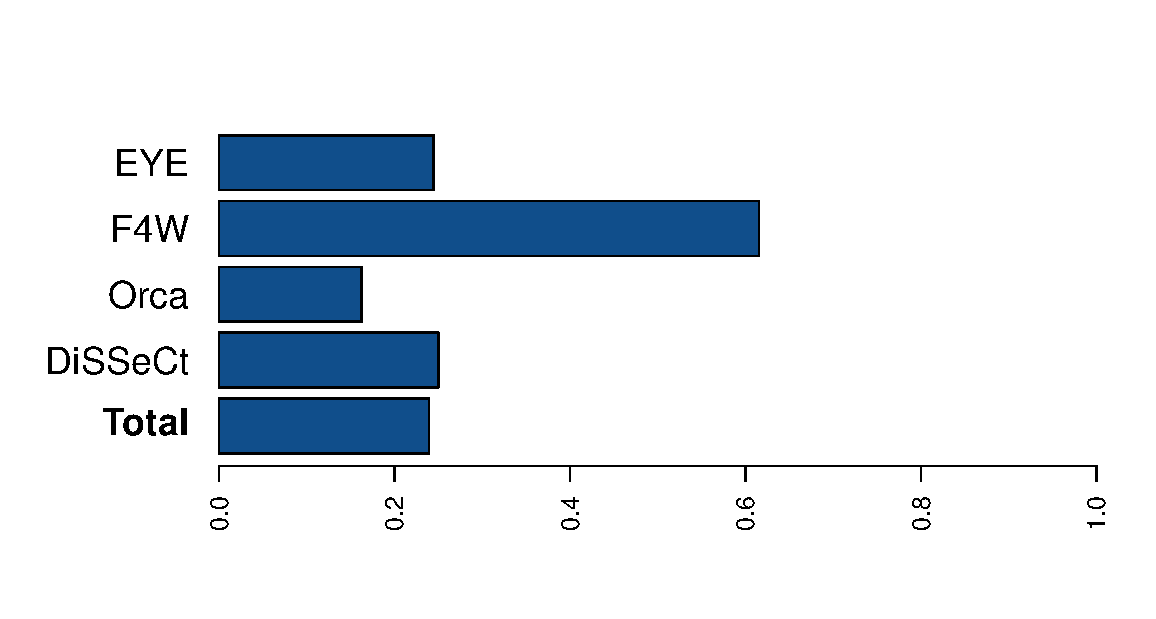
\includegraphics[width=\linewidth]{Rplot10.pdf}
%         \caption{Share of files containing built-ins causing conflicting interpretations in
%  files containing built-ins. Only in a quarter of all files containing built-ins 
%  these occur with deeply nested universals. }
%     \end{minipage}% <- sonst wird hier ein Leerzeichen eingefügt
%     \hfill
%     \begin{minipage}[t]{0.49\linewidth}
%         \centering
%         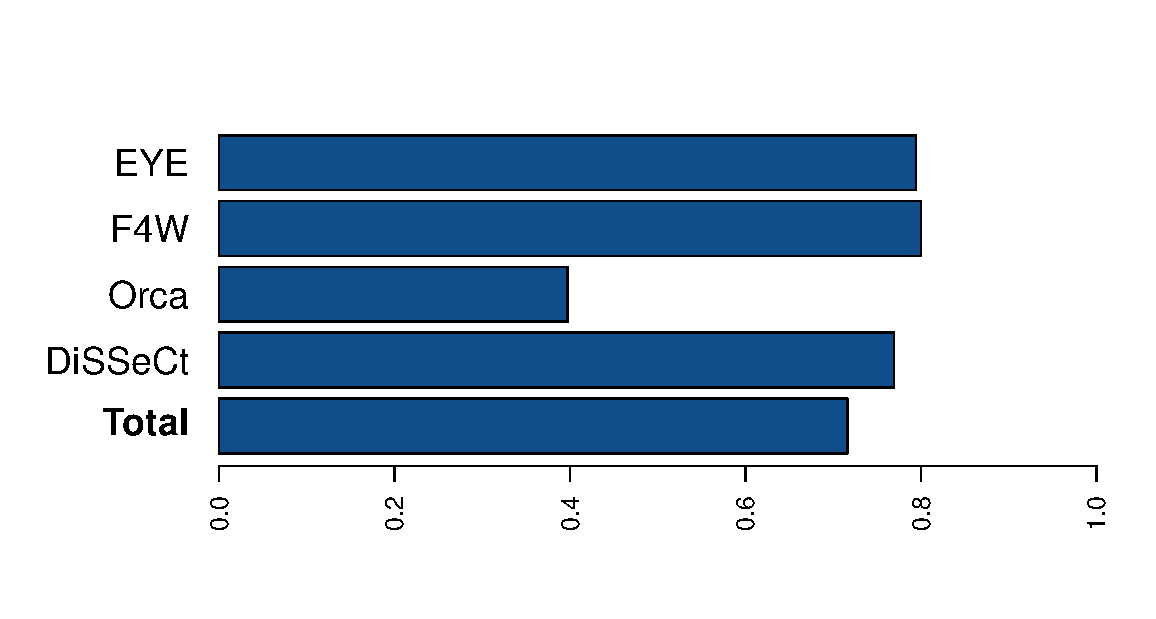
\includegraphics[width=\linewidth]{Rplot12.pdf}
%         \caption{Share of files causing conflicting interpretations in
%  files which have nested expressions. 72\% of the files containing nesting are interpreted differently by both reasoners.}
%     \end{minipage}
% \end{figure}
% 
% \begin{figure}
%  \includegraphics[width=\textwidth]{2zusammen.pdf}
%  \caption{Share of files causing conflicting interpretations in
%  files which have nested expressions. 72\% of the files containing nesting are interpreted differently by both reasoners.
% \label{222}}
% \end{figure}
% 
% How are these
% cases distributed within the datasets? 
% To find the different cases we have added two features to our implementation: for every formula parsed, there are evaluation functions providing a number indicating 
% for Cwm's interpretations, how deep the most deeply nested universal quantifiers occur and which variables are quantified under these deeply nested quantifiers.
% If universal quantifiers only occur on top level, the \emph{depth} is one, if a
% universal quantifier occurs in a formula expression which is a direct component of the overall formula, the depth is two, this is for example the case 
% for the formula in Listing~\ref{F4Wcwm}, if a universal quantifier occurs in a formula expression which is component of another formula expression which is a direct component 
% of the overall formula, the depth is three, etc.
% %We do this kind of assignment to determine whether a the formula expressions of a proof contain nested constructions or only rather simple rules as in the example above.
% %
% This assignment enables the above mentioned classification: if a proof has depth two, we know that the proof steps do not lead to formulas with a depth higher than one. 
% If the depth is more than two, we can look up the variables nested more deeply to decide whether they are used in connection with built-in functions or not.


Following this classification, the results of our tests are displayed in Figure~\ref{result2}.
For the overall dataset (last line) half (51\%) of the conflicts between reasoning results occur only because of the different interpretations of proofs. 
As discussed these can be considered as rather harmless. % since they these universal variables normally occur in connection with \texttt{r:gives}.
The next bigger group of differences occurs in connections with built-in functions (31\%). 
Here, not all, but some of the conflicts are unavoidable,
since some built-in functions are not supported by all reasoners. The last group of conflicts (13\%), caused by the simple use of nested graphs or rules 
without direct involvement of built-in functions or proof predicates,  is the most dangerous: while users employing built-in functions are often
aware that the support of these could be limited to one reasoner and therefore also check carefully when they want to switch to a different one, 
this is not the case here. If nested rules and graphs are used without
any special predicates, it is normally expected that the reasoning results from formulas containing these constructions do not differ between reasoners. 
%with these files should be independent of the reasoner. 
The user  has no reason to do extra compatibility checks.

Whether these cases occur depends on the use case: 
In the DiSSeCt dataset, such cases do not occur. This has to do with the fact that the use case here is the test for constraints on \rdf data, ie data 
without formula expressions 
or rules. 
The constraints themselves and the results
are plain \rdf and there is always only one reasoning run applied in order to find constraint violations. In contrast, the Facts4Workers dataset contains
many constructs similar to the one displayed in Listing~\ref{F4W} and does therefore have a rather high occurrence of cases belonging to the last category (33\%).

\begin{figure}\centering
 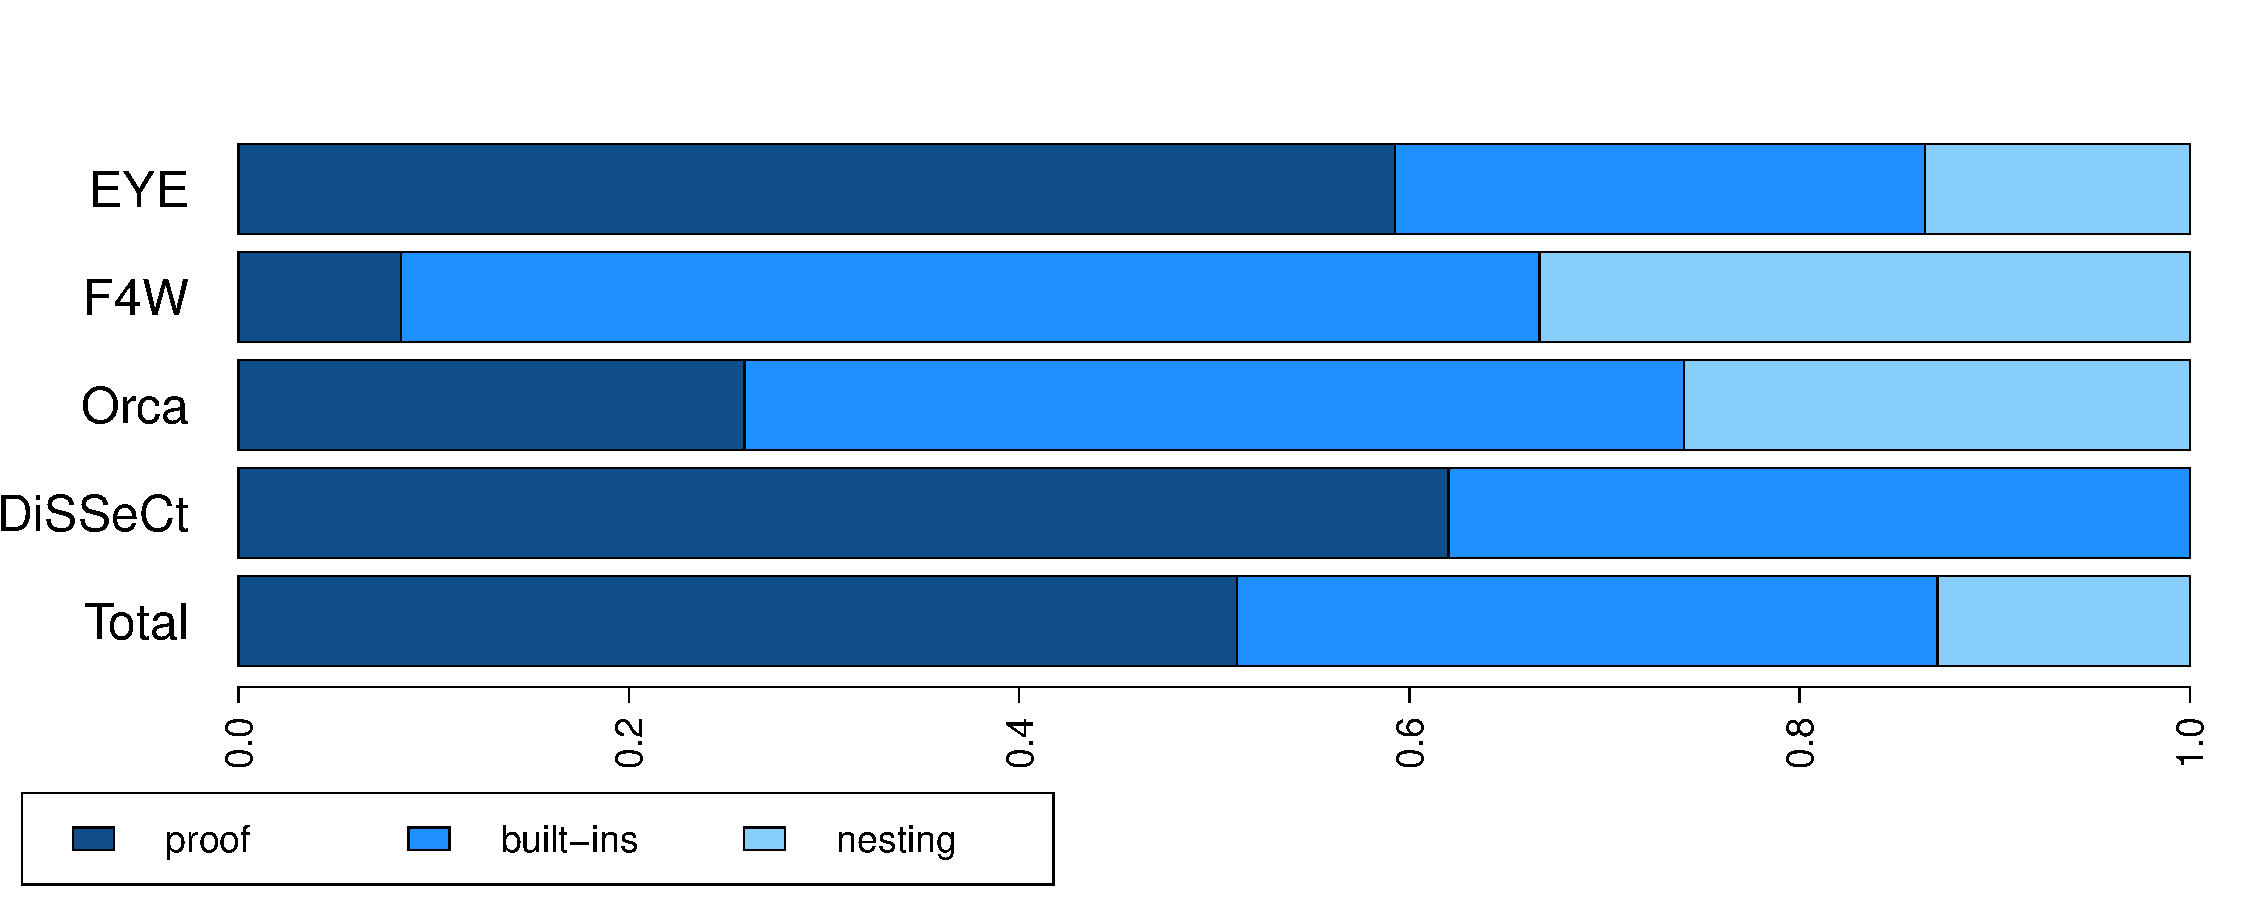
\includegraphics[width=0.9\textwidth]{Rplot22.pdf}
 \caption{Distribution of different cases causing conflicting interpretations by the reasoners Cwm and EYE.\label{result2}}
\end{figure}
% \begin{figure}
% \begin{center}
% \begin{tabular}{lccccccc}
% Dataset & \# of  & \multicolumn{6}{c}{reasons} \\
%         & diff               & \multicolumn{2}{c}{proof}&\multicolumn{2}{c}{built-ins}&\multicolumn{2}{c}{nested graphs}\\
%         &                & \# & \% & \# & \% & \# & \% \\
% \hline
%  EYE  &81 &  48 & 59\% & 22 & 27\%& 11& 14\%\\
%  F4W  &12 &  1 & 8\%& 7 & 58\%& 4& 33\% \\
%  ORCA  &27 & 7 & 26\%&13 & 48\% & 7& 26\% \\
%  DiSSeCt &50& 31 & 62\%&19& 38\%&-&-  \\
%  \hline
% \end{tabular}
% \end{center}
% \caption{Distribution of difference classes per dataset.\label{res2}}
% \end{figure}
% 
% \begin{figure}
% \begin{center}
% \begin{tabular}{lC{1.5cm}C{1.5cm}C{1.5cm}}
% \hline\hline
% Dataset &  \multicolumn{3}{c}{Occurence of reasons for conflicts (in \%)} \\
%         &proof&built-ins&nested graphs\\
% \hline
%  EYE  &  59& 27&  14\\
%  F4W  &   8& 58&  33 \\
%  ORCA  &  26& 48 &  26 \\
%  DiSSeCt & 62& 38&-  \\
%  \hline
%  All & 51&36 &13\\
%  \hline \hline
% \end{tabular}
% \end{center}
% \caption{Distribution of different cases causing conflicting interpretations by the reasoners Cwm and EYE.\label{res2}}
% \end{figure}
